% Template for Cogsci submission with R Markdown

% Stuff changed from original Markdown PLOS Template
\documentclass[10pt, letterpaper]{article}

\usepackage{cogsci}
\usepackage{pslatex}
\usepackage{float}
\usepackage{caption}

% amsmath package, useful for mathematical formulas
\usepackage{amsmath}

% amssymb package, useful for mathematical symbols
\usepackage{amssymb}

% hyperref package, useful for hyperlinks
\usepackage{hyperref}

% graphicx package, useful for including eps and pdf graphics
% include graphics with the command \includegraphics
\usepackage{graphicx}

% Sweave(-like)
\usepackage{fancyvrb}
\DefineVerbatimEnvironment{Sinput}{Verbatim}{fontshape=sl}
\DefineVerbatimEnvironment{Soutput}{Verbatim}{}
\DefineVerbatimEnvironment{Scode}{Verbatim}{fontshape=sl}
\newenvironment{Schunk}{}{}
\DefineVerbatimEnvironment{Code}{Verbatim}{}
\DefineVerbatimEnvironment{CodeInput}{Verbatim}{fontshape=sl}
\DefineVerbatimEnvironment{CodeOutput}{Verbatim}{}
\newenvironment{CodeChunk}{}{}

% cite package, to clean up citations in the main text. Do not remove.
\usepackage{cite}

\usepackage{color}

% Use doublespacing - comment out for single spacing
%\usepackage{setspace}
%\doublespacing


% % Text layout
% \topmargin 0.0cm
% \oddsidemargin 0.5cm
% \evensidemargin 0.5cm
% \textwidth 16cm
% \textheight 21cm

\title{Children seek additional visual information when it is useful for
language comprehension}


\author{ {\large \bf Kyle MacDonald}$^1$ (kylem4@stanford.edu), {\large \bf Virginia Marchman}$^1$ (marchman@stanford.edu),  \\ {\large \bf Anne Fernald}$^1$ (afernald@stanford.edu), {\large \bf Michael C. Frank}$^1$ (mcfrank@stanford.edu) 
  \\ $^1$ Department of Psychology Stanford University}

\begin{document}

\maketitle

\begin{abstract}
Language comprehension is multisensory and interactive. Skilled
listeners rapidly integrate information from both the visual and the
linguistic signal to reach a candidate interpretation. But the quality
of the available information varies across contexts, e.g., speech in
noisy environments. Here, we test the hypothesis that listeners adapt
the dynamics of gaze to seek visual information when it supports
comprehension. In E1, we show that adults (n=31) and children (n=40, 3-5
y.o.) delayed eye movements away from a speaker's face while processing
speech in noise. Interestingly, this delay resulted in more information
accumulation, higher accuracy, and fewer random responses. In E1, we
show that adults (n=31) and children (n=38, 3-5 y.o.) do not delay eye
movements away from a speaker who provides a post-nominal gaze cue.
These results suggest that listeners adapt to the processing demands of
different contexts and seek additional visual information to support
real-time language comprehension.

\textbf{Keywords:}
eye movements; language processing; information-seeking; speech in
noise; social cue processing
\end{abstract}

\section{Introduction}\label{introduction}

Real-time language comprehension is multimodal. As skilled listeners, we
continually integrate information from both the visual and the
linguistic signal to understand what others are saying. A classic
demonstration of this integration process is the ``McGurk effect'' where
a speaker's mouth movements suggest one sound while their acoustic
output suggests another. This conflict results in the listener
perceiving a third, intermediate sound (J. MacDonald \& McGurk, 1978).
Findings such as these have inspired prominent theories of speech
perception (McClelland, Mirman, \& Holt, 2006) and lexical processing
(M. C. MacDonald \& Seidenberg, 2006; Smith, Monaghan, \& Huettig, 2017)
that argue for the fundamental role of \emph{interactive} processes --
where listeners process information from multiple sources in parallel.
Moreover, empirical work on speech perception shows that adults are
better able to ``recover'' linguistic information in noisy contexts when
they have visual access to a speaker's face (Erber, 1969)

However, the usefulness of integrating visual information with the
linguistic signal varies depending on features of the listener/language
and features of the context. Consider the case of processing a
visual-manual language like American Sign Language (ASL). Here, the
value of allocating visual fixations to the language source (the signer)
is high since all of the language-relevant information is available in
that fixation location. In our prior work, we showed evidence that
ASL-learners were more sensitive to the value of eye movements in a
visual language, choosing to prioritize information accumulation and
accuracy over and above speed when deciding to shift gaze away from
signer (K. MacDonald, Blonder, Marchman, Fernald, \& Frank, 2017). To
explain these differences, we proposed an information-seeking account
inspired by goal-based theories of vision (Hayhoe \& Ballard, 2005):
that signers adapted the dynamics of gaze during lexical access to
produce behaviors that would better achieve the goal of accurate
language comprehension.

However, there is an abundance of population-level differences between
children learning ASL and children learning spoken English. Thus, we
thought it was critical to isolate the underlying factor of interest --
i.e., features of the processing context that modulate the value of
different gaze patterns -- to test the predictions of our
information-seeking account. Here, we ask whether our proposal
generalizes to (1) processing speech in noise and (2) processing speech
accompanied by a visual cue to reference (eye gaze).

We hypothesized that processing speech in noisy environments would make
the auditory signal less useful, and in turn make the visual signal more
valuable. Moreover, we chose social cue processing because a speaker who
gazes at an object becomes a more informative fixation target, and
social-pragmatic theories of language acquisition emphasize the role of
processing social cues for early language acquisition (Clark, 2009).

Our key prediction is that increasing the value of fixating on the
speaker (noise and gaze conditions) will make gaze shifts away from the
language source less valuable, which in turn will lead listeners to
delay seeking a named referent until they have accumulated additional
visual information.

\section{Experiment 1}\label{experiment-1}

E1 asks whether our information-seeking account generalizes to a novel
and ecologically valid processing context -- speech in noise. We
recorded eye movements during a real-time language comprehension task
where children and adults processed familiar sentences (e.g., ``Where's
the ball?'') while looking at a simplified visual world with three
fixation targets (see Fig 1). Using a within-participants design, we
manipulated the signal-to-noise ratio of the auditory information by
convolving the linguistic signal with brown noise. We predicted that
processing speech in noise would increase the value of fixating on the
speaker, causing listeners to gather additional information before
generating a shift to the named referent even after the target word
began unfolding in time.

To quantify evidence for this prediction, we compare the Accuracy and
Reaction Times (RTs) of participants' first shift after target noun
onset across the noise and clear contexts. We also present two
model-based analyses that link the observable behavior to underlying
psychological constructs of interest. First, we use an exponentially
weighted moving average (EWMA) method (Vandekerckhove \& Tuerlinckx,
2007) to categorize gaze shifts as language-driven or random (a measure
that we label the ``guessing'' parameter). In contrast to the standard
RT/Accuracy analysis, the EMWA allows us to quantify participants'
willingness to generate gaze shifts after noun onset but before
collecting sufficient information to seek the named referent.

Next, we use drift-diffusion models (DDMs) (Ratcliff \& Childers, 2015)
to ask whether the behavioral differences in Accuracy and RT are driven
by a more cautious responding strategy (indexed by a parameter called
boundary separation) or by more efficient information processing
(indexed by a parameter called drift rate). We predicted that processing
speech in noise would make participants less likely to shift before
collecting sufficient information, leading to a higher guessing
parameter estimate in the EWMA and a higher boundary separation estimate
in the DDM.

\begin{CodeChunk}
\begin{figure}[tb]

{\centering 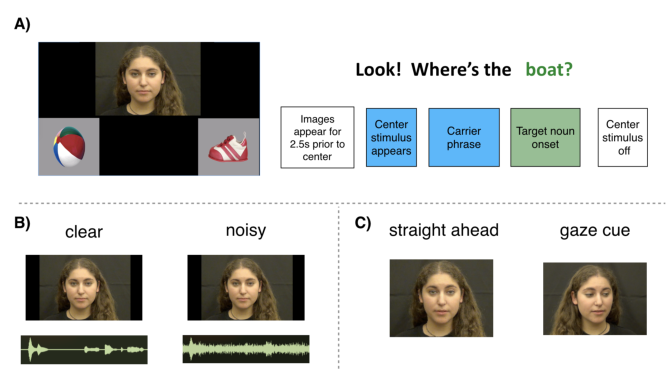
\includegraphics[width=0.95\linewidth]{figs/stimuli_plot-1} 

}

\caption[Stimuli for E1 and E2]{Stimuli for E1 and E2. Panel A shows the layout of the three fixation locations (speaker, target, and distracter), and the timecourse of a single trial. Panel B shows a visual representation of the clear and noisy waveforms used in E1. Panel C shows the gaze manipulation used in E2.}\label{fig:stimuli_plot}
\end{figure}
\end{CodeChunk}

\begin{CodeChunk}
\begin{figure*}[t]

{\centering 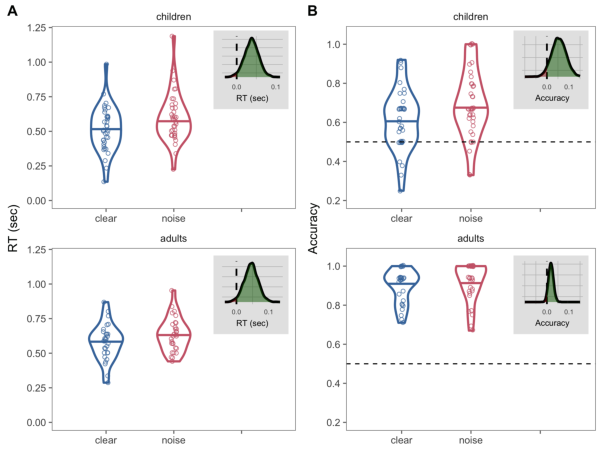
\includegraphics[width=0.7\linewidth]{figs/noise_acc_rt_e1_plot-1} 

}

\caption[Behavioral results from E1]{Behavioral results from E1. Panel A shows violin plots representing the distribution of RTs for each participant in each condition. Each black point represents a participant. The dark red points represent the most likely estimate for the group mean with the error bars showing the 95\% Highest Density Interval. The grey inset plot shows the full posterior distribution of the plausible RT difference across conditions with the vertical dashed line representing the null value of zero condition difference. The green shading represents estimates in the predicted direction and above the null value while the red shading represents estimates below the null. Panel B shows the same information but for First Shift Accuracy.}\label{fig:noise_acc_rt_e1_plot}
\end{figure*}
\end{CodeChunk}

\subsection{Method}\label{method}

\subsubsection{Participants}\label{participants}

Participants were native, monolingual English-learning children (\(n=\)
39; 22 F, 17 M) and adults (\(n=\) 31; 22 F, 9 M). All participants had
no reported history of developmental or language delay and normal
vision. 14 participants (11 children, 3 adults) were run but not
included in the analysis because either the eye tracker falied to
calibrate or the participant did not complete the task.

\subsubsection{Stimuli}\label{stimuli}

\emph{Linguistic stimuli.} The stimuli were recorded in a sound-proof
room and featured two female speakers who used natural child-directed
speech and said one of two phrases: ``Hey! Can you find the (target
word)'' or ``Look! Where's the (target word) -- see panel A of Fig 1.
The target words were: ball, bunny, boat, bottle, cookie, juice,
chicken, and shoe. The target words varied in length (shortest = 411.68
ms, longest = 779.62 ms) with an average length of 586.71 ms.

\emph{Noise manipulation}. To create the noisy stimuli, we convolved the
recordings with Brown noise using the Audacity audio editor. The average
signal-to-noise ratio\footnote{The ratio of signal power to the noise
  power, with values greater than 0 dB indicating more signal than
  noise.} in the noise condition was 2.87 dB compared to the clear
condition, which was 35.05 dB.

\emph{Visual stimuli.} The image set consisted of colorful digitized
pictures of objects presented in fixed pairs with no phonological
overlap between the target and the distractor image (cookie-bottle,
boat-juice, bunny-chicken, shoe-ball). The side of the target picture
was counterbalanced across trials.

\subsubsection{Design and procedure}\label{design-and-procedure}

Participants viewed the task on a screen while their gaze was tracked
using an SMI RED corneal-reflection eye-tracker mounted on an LCD
monitor, sampling at 60 Hz. The eye-tracker was first calibrated for
each participant using a 6-point calibration. On each trial,
participants saw two images of familiar objects on the screen for two
seconds before the center stimulus appeared (see Fig 1). Then they
processed the target sentence -- which consisted of a carrier phrase, a
target noun, and a question -- followed by two seconds without language
to allow for a response. Child participants saw 32 trials (16 noise
trials; 16 clear trials) with several filler trials interspersed to
maintain interest. Adult participants saw 64 trials (32 noise; 32
clear).

\subsection{Results and Discussion}\label{results-and-discussion}

\subsubsection{Analysis plan}\label{analysis-plan}

First, we present behavioral analyses of First Shift Accuracy and
Reaction Time (RT). RT corresponds to the latency to shift away from the
central stimulus to either picture measured from the onset of the target
noun. (Note that we log-transformed all RTs for the statistical models).
Accuracy corresponds to whether the participant's first gaze shift
landed on the target or the distracter picture. We used the
\texttt{rstanarm} (Gabry \& Goodrich, 2016) package to fit Bayesian
mixed-effects regression models. The mixed-effects approach allowed us
to model the nested structure in our data (multiple trials for each
participant; and a within-participants manipulation) by including random
intercepts for each participant and item, and a random slope for each
item and noise condition. We used Bayesian estimation to quantify
uncertainty in our point estimates, which we communicate using 95\%
Highest Density Intervals (HDI), which provides a range of credible
values given the data and model. All analysis code can be found in the
online repository for this project:
\url{https://github.com/kemacdonald/speed-acc/R/analysis}.

Next, we present the two model-based analyses -- the EWMA and DDM. The
goal of these models is to move beyond a description of the data and map
behavioral differences in eye movements to underlying psychological
variables. The EWMA method models changes in random shifting behavior as
a function of RT. For each participant, the model classifies the
proportion of shifts that were likely to be language-driven as opposed
to random responding, which we call the \emph{guessing} parameter.

After fitting the EWMA, we took the shifts that were categorized as
language-driven and fit a hierarchical Bayesian drift-diffusion model
(HDDM). This model quantifies differences in separable parameters of the
underlying decision process that lead to different patterns of behavior.
The model assumes that people accumulate noisy evidence in favor of one
alternative with a response generated when the evidence crosses a
pre-defined decision threshold. Here, we focus on two parameters of
interest: \textbf{boundary separation}, which indexes the amount of
evidence gathered before generating a response (higher values suggest
more cautious responding) and \textbf{drift rate}, which indexes the
amount of evidence accumulated per unit time (higher values suggest more
efficient processing).

\subsubsection{Behavioral analyses}\label{behavioral-analyses}

\textbf{RT.} To make RTs more suitable for modeling on a linear scale,
we analyzed responses in log space with the final model specified as:
\texttt{$log(RT) \sim noise\_condition + age\_group + (sub\_id + noise\_condition \mid item)$}.
Panel A of Figure 2 shows the full RT data distribution, the estimates
of condition means, and the full posterior distribution of the estimated
difference between the noise and clear conditions. Both children and
adults were slower to identify the target in the noise condition
(Children \(M_{noise}\) = 0.5 ms; Adult \(M_{noise}\) = 0.6 ms), as
compared to the clear condition (Children \(M_{clear}\) = 0.46 ms; Adult
\(M_{clear}\) = 0.55 ms). RTs in the noise condition were 41.73 ms
slower on average, with a 95\% HDI from 1.19 ms to 82.26 ms that did not
include the null value of zero condition difference.

\textbf{Accuracy.} Next, we modeled adults' and children's first shift
accuracy using a mixed-effects logistic regression with the same
specifications (see Panel B of Fig 2). Both groups were more accurate
than a model of random responding (null value of \(0.5\) falling well
outside the lower bound of the 95\% HDI for all group means). Adults
were more accurate (\(M_{adults} =\) 90\%) than children
(\(M_{children} =\) 62\%). The key result is that both groups showed
evidence of higher accuracy in the noise condition (Children
\(M_{noise}\) = 67\%; Adult \(M_{noise}\) = 92\%) as compared to the
clear condition (Children \(M_{clear}\) = 62\%; Adult \(M_{clear}\) =
90\%). Accuracy in the noise condition was 4\% higher on average, with a
95\% HDI from 0\% to 11\%. Note that the null value of zero difference
falls at the very edge of the 95\% HDI such that 95\% of the credible
values fall below the null, providing evidence for higher accuracy in
the noise condition.

\subsubsection{Model-based analyses}\label{model-based-analyses}

\begin{table}[b]
\centering
\begin{tabular}{llr}
  \hline
Exp. & Contrast & Estimate (95\% HDI) \\ 
  \hline
E1 & adults-children & 0.46 [0.43, 0.49] \\ 
  E1 & noise-clear & 0.12 [0.07, 0.17] \\ 
   \hline
E2 & adults-children & 0.45 [0.42, 0.48] \\ 
  E2 & gaze-straight\_ahead & -0.03 [-0.07, 0] \\ 
   \hline
\end{tabular}
\caption{EWMA results for E1 and E2. The guessing parameter refers to the proportion of gaze shifts classified as random vs. language-driven with higher values indicating more random responding. Estimate refers to the difference between condition or age group.} 
\end{table}

\textbf{EWMA.} Table 1 shows estimates of the age and condition
contrasts in the EWMA model. Critically, processing speech in noise
caused both adults and children to produce a higher proportion of
language-driven shifts with the 95\% HDI excluding the null value. This
pattern of evidence suggests that the noise condition led participants
to increase visual fixations to the language source, leading them to
generate fewer exploratory, random shifts before accumulating sufficient
information to respond accurately.

\textbf{HDDM.} Figure 3 shows the HDDM results. Children had lower drift
and boundary separation as compared to adults, suggesting that children
were less efficient and less cautious in their responding. The noise
manipulation only affected the boundary separation parameter, with
higher estimates in the noisy processing context across both age groups.
This result suggests that participants' in the noise condition
prioritized information accumulation before generating an eye movement,
leading to higher accuracy. Moreover, the high overlap in estimates of
drift rate suggests that participants were integrating the visual and
auditory signals to achieve similar levels of processing efficiency.

\begin{CodeChunk}
\begin{figure}[t]

{\centering 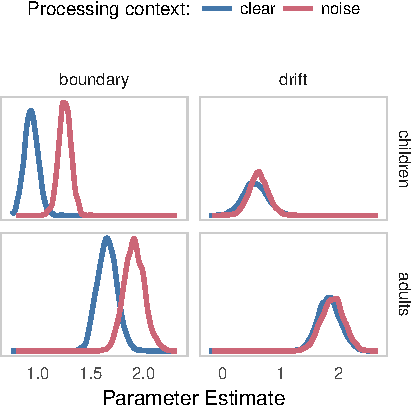
\includegraphics[width=0.7\linewidth]{figs/hddm_plot_noise-1} 

}

\caption[HDDM results E1]{HDDM results E1.}\label{fig:hddm_plot_noise}
\end{figure}
\end{CodeChunk}

Togher, the behavioral and EWMA/HDDM results provide converging support
for predictions of our information-seeking account: that processing
speech in noise caused listeners to seek additional visual information
to support language comprehension. Moreover, we observed a strikingly
similar pattern of behavior in children and adults, with both groups
producing more language-driven shifts and prioritizing accuracy over
speed in the noisier context. These data have interesting parallels to
recent work by McMurray, Farris-Trimble, \& Rigler (2017), showing that
adults Cochlear Implants users, who consistently process degraded
auditory input, will delay lexical access and wait until substantial
information has accumulated. This process is in contrast to the
``immediate competition'' model of word recognition where listeners
activate candidate meanings from word onset.

Degrading the auditory signal is just one way ecologically valid way to
make the visual information more useful. However, there are many other
processing contexts where features of the visual world provide
particularly useful information for language comprehension. In E2, we
test our account in another context -- processing speech accompanied by
a visual cue to reference, a speaker's eye gaze.

\begin{CodeChunk}
\begin{figure*}[tb]

{\centering 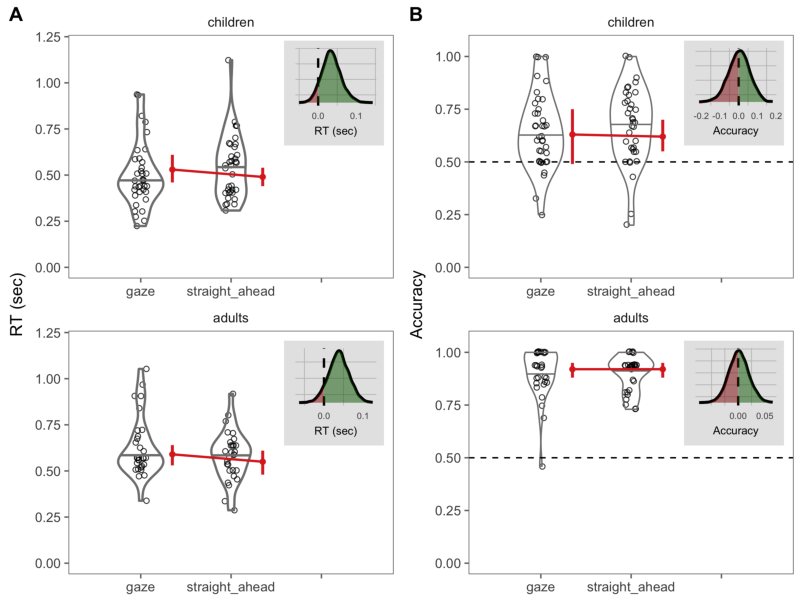
\includegraphics[width=0.7\linewidth]{figs/gaze_acc_rt_e2_plot-1} 

}

\caption[Behavioral results from E2]{Behavioral results from E2. All plotting conventions are the same as in Figure 2.}\label{fig:gaze_acc_rt_e2_plot}
\end{figure*}
\end{CodeChunk}

\section{Experiment 2}\label{experiment-2}

In E2, we ask whether increasing the information value of the speaker as
a target for visual fixations will produce a similar shift in the
dynamics of gaze patterns during language comprehension. We compared the
timing and accuracy of adults and children's eye decisions to shift away
from a language source across two processing contexts: speech with and
without a social cue to reference (eye gaze). We hypothesized that the
gaze cue would cause listeners to delay their response and accumulate
more information, leading to more accurate responses. Our key model
predictions were that listeners in the gaze condition would produce a
higher proportion of language-driven shifts as indexed by the EWMA
output and higher boundary parameter estimates in the HDDM.

\subsection{Method}\label{method-1}

\subsubsection{Participants}\label{participants-1}

Participants were native, monolingual English-learning children (\(n=\)
38; 19 F, 19 M) and adults (\(n=\) 31; 22 F, 9 M). All participants had
no reported history of developmental or language delay and normal
vision. 12 participants (9 children, 3 adults) were run but not included
in the analysis either because the eye tracker falied to calibrate or
the participant did not complete the task.

\subsubsection{Stimuli}\label{stimuli-1}

The audio stimuli were identical to the stimuli used in E1. We included
a new center fixation stimulus type: a video of a speaker who produced a
post-nominal gaze cue (see Fig 1). The onset of gaze occurred at the end
of each target noun. We chose a post-nominal cue to give us the best
opportunity to detect whether participants would delay shifting away
from the speaker to gather additional visual information before seeking
the named referent.

\subsubsection{Design and procedure}\label{design-and-procedure-1}

The design was identical to E1. Child participants saw 32 trials (16
gaze; 16 straight ahead) with several filler trials interspersed to
maintain interest. Adult participants saw 64 trials (32 gaze; 32
straight ahead). The gaze manipulation was presented in a blocked design
with the order of block counterbalanced across participants.

\subsection{Results and Discussion}\label{results-and-discussion-1}

\subsubsection{Behavioral analyses}\label{behavioral-analyses-1}

\textbf{RT.} Panel A of Figure 4 shows the full RT data distribution,
the estimates of condition means, and the full posterior distribution of
the estimated difference between the gaze and straight-ahead conditions.
Both age groups responded with similar speed with the average difference
in RTs in the gaze condition was 3.81 ms, with a 95\% HDI from -28.76 ms
to 37.2 ms that did included the null value of zero condition
difference.

\textbf{Accuracy.} Next, we quantified first shift accuracy. Overall,
both groups were more accurate than a model of random behavior (null
value of \(0.5\) falling well outside the lower bound of all group
means). Adults were more accurate (\(M_{adults} =\) 90\%) compared to
children (\(M_{children} =\) 62\%). And both groups were equally
accurate across the gaze conditions with the average difference being
-2\%, with a 95\% HDI from -9\% to 2\% centered around the null value of
zero condition difference.

\subsubsection{Model-based analyses}\label{model-based-analyses-1}

\textbf{EWMA.} Table 1 shows the interval of credible parameter
estimates for the age and condition contrasts in the EWMA model. There
was some evidence that the presence of gaze increased the proportion of
shifts classified as language-driven. This pattern of results suggests
that the gaze condition led listeners to sustain visual attention to the
language source, leading them to generate fewer early random gaze
shifts.

\textbf{HDDM.} Figure 4 shows the HDDM results. Children had lower drift
and boundary separation, replicating a result from E1. For children,
there was high overlap in both parameters across the two gaze contexts.
But, for adults, there was some evidence that the presence of gaze
increased boundary separation and decreased drift. This pattern suggests
that, in the subset of ``language-driven'' shifts, adults accumulated
more information before responding in the gaze condition, but achieved
comparable accuracy in the straight-ahead condition by processing the
stimuli more efficiently.

\begin{CodeChunk}
\begin{figure}[t]

{\centering 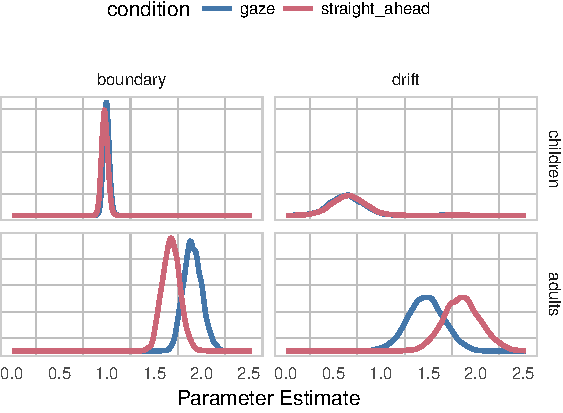
\includegraphics[width=0.7\linewidth]{figs/hddm_plot_gaze-1} 

}

\caption[HDDM results E2]{HDDM results E2.}\label{fig:hddm_plot_gaze}
\end{figure}
\end{CodeChunk}

{[}TODO: short wrap up of gaze results.{]}

\section{General Discussion}\label{general-discussion}

Language comprehension in grounded contexts involves integrating the
visual and linguistic signals. But the value of visual information can
vary depending on what information is available to the listener and the
quality of the incoming language. Here, we tested two predictions of an
information-maximization account of eye movements during language
processing that we proposed in K. MacDonald et al. (2017). The account
aimed to explain population-level differences in the dynamics of gaze
between children learning ASL and children learning spoken English.

In E1, we showed that children and adults adapt to processing speech in
noise by producing slower but more accurate gaze shifts away from a
speaker. Both groups also showed evidence of prioritizing information
accumulation over speed (HDDM) while producing more language driven
shifts (EWMA). It is interesting that listeners were able to achieve
higher accuracy in the more challenging, noisy context. In E2, adults
and children did not show strong evidence of delaying gaze shifts to
wait for a post-nominal cue to reference. However, for adults, the
model-based analyses suggest that the gaze manipulation did reduce the
rate of early random shifting (EWMA) and increased the amount of
information accumulated before responding (HDDM).

Together, these results represent a confirmatory test of our
information-seeking account (E1) and place a limit on the scope of the
adaptive response (E2). That is, when the linguistic signal is degraded,
eye movements to seek visual language-relevant information become more
useful, shifting the dynamics of gaze. However, if the linguistic signal
is clear, then the listener does not have to delay seeking a named
referent to gather a post-nominal visual cue and is free to look
elsewhere while they listen.

These results connect ideas from several rich research traditions.
First, work on language-mediated visual attention shows that adults and
children rapidly shift gaze upon hearing the name of an object in the
visual scene (Allopenna, Magnuson, \& Tanenhaus, 1998; Tanenhaus,
Spivey-Knowlton, Eberhard, \& Sedivy, 1995). The speed and consistency
of this response has led to debates about whether language-mediated gaze
shifts are automatic as opposed to under the control of the listener.
While we do claim that listeners in our task have explicit access to the
underlying decision process, our findings show that the dynamics of gaze
during lexical access adapt to the information features of the context.
This finding parallels recent work by McMurray et al. (2017), showing
that adults with Cochlear Implants, who consistently process degraded
auditory input, will delay the process of lexical access, waiting to
begin until substantial information has accumulated.

Second, empirical work on vision during natural tasks shows that people
overwhelmingly prefer to look at \emph{goal-relevant} locations -- e.g.,
an upcoming obstacle while walking (Hayhoe \& Ballard, 2005). These
accounts inspired our prediction that gaze dynamics during language
comprehension should adapt to the value of different fixation behaviors
with respect to the listener's goal of rapid language processing. And
third, work on effortful listening shows that listeners generate
compensatory responses (e.g., increases in attention and working memory)
within ``challenging'' comprehension contexts such as processing noisy
or accented speech (Van Engen \& Peelle, 2014). These accounts predict
that our young listeners might compensate for the reduced quality of the
auditory signal by allocating gathering additional visual information.

This work has several important limitations that we hope will pave the
way for future work. Here, we chose to focus on a single decision about
visual fixation to provide a window onto the underlying dynamics of
decision-making across different processing contexts. However, the
decision to shift away from a language is just one of the \emph{many}
decisions that listeners make while processing language in real-time.
Moreover, our micro-level analysis does not consider the rich gaze
patterns that occur before this decision. In our future work, we aim to
quantify changes in the dynamics of gaze across the full sentence
processing context. Finally, we used a simple visual world, with only
three places to look, and very simple linguistic stimuli, especially for
the adults. Thus it remains an open question how these results might
scale up to more complex language information and visual environments.

We designed these experiments to test our information-maximization
proposal in the domain of familiar language comprehension. However, we
think the account is more general. And we are interested in applying
this framework -- the use of in-depth analyses of the micro-level
decisions about visual fixation -- to the early language
\emph{acquisition} context. Consider that early in language learning
children are acquiring novel word-object links while also learning about
visual object categories. Both of these tasks produce goals that should
shape children's decisions about visual fixation, e.g., changing the
information value of looks to a speaker vs.~looks to an object. More
generally, we think that these results contribute to recent theoretical
work emphasizing the need for goal-based accounts of eye movements
during language comprehension (Salverda, Brown, \& Tanenhaus, 2011). And
we hope that our approach offers a way forward to explain fixation
behaviors across a wider variety of populations, processing contexts,
and during different stages of language learning.

\section{Acknowledgements}\label{acknowledgements}

We are grateful to the families who participated in this research.
Thanks to Tami Alade and Hannah Slater for help with data collection.
This work was supported by an NSF GRFP to KM.

\section{References}\label{references}

\setlength{\parindent}{-0.1in} \setlength{\leftskip}{0.125in} \noindent

\hypertarget{refs}{}
\hypertarget{ref-allopenna1998tracking}{}
Allopenna, P. D., Magnuson, J. S., \& Tanenhaus, M. K. (1998). Tracking
the time course of spoken word recognition using eye movements: Evidence
for continuous mapping models. \emph{Journal of Memory and Language},
\emph{38}(4), 419--439.

\hypertarget{ref-clark2009first}{}
Clark, E. V. (2009). \emph{First language acquisition}. Cambridge
University Press.

\hypertarget{ref-erber1969interaction}{}
Erber, N. P. (1969). Interaction of audition and vision in the
recognition of oral speech stimuli. \emph{Journal of Speech and Hearing
Research}, \emph{12}(2), 423--425.

\hypertarget{ref-gabry2016rstanarm}{}
Gabry, J., \& Goodrich, B. (2016). Rstanarm: Bayesian applied regression
modeling via stan. r package version 2.10. 0.

\hypertarget{ref-hayhoe2005eye}{}
Hayhoe, M., \& Ballard, D. (2005). Eye movements in natural behavior.
\emph{Trends in Cognitive Sciences}, \emph{9}(4), 188--194.

\hypertarget{ref-macdonald1978visual}{}
MacDonald, J., \& McGurk, H. (1978). Visual influences on speech
perception processes. \emph{Attention, Perception, \& Psychophysics},
\emph{24}(3), 253--257.

\hypertarget{ref-macdonald2017info}{}
MacDonald, K., Blonder, A., Marchman, V. and, Fernald, A., \& Frank, M.
C. (2017). An information-seeking account of eye movements during spoken
and signed language comprehension. In \emph{Proceedings of the 39th
annual conference of the cognitive science society}.

\hypertarget{ref-macdonald2006constraint}{}
MacDonald, M. C., \& Seidenberg, M. S. (2006). Constraint satisfaction
accounts of lexical and sentence comprehension. \emph{Handbook of
Psycholinguistics}, \emph{2}, 581--611.

\hypertarget{ref-mcclelland2006there}{}
McClelland, J. L., Mirman, D., \& Holt, L. L. (2006). Are there
interactive processes in speech perception? \emph{Trends in Cognitive
Sciences}, \emph{10}(8), 363--369.

\hypertarget{ref-mcmurray2017waiting}{}
McMurray, B., Farris-Trimble, A., \& Rigler, H. (2017). Waiting for
lexical access: Cochlear implants or severely degraded input lead
listeners to process speech less incrementally. \emph{Cognition},
\emph{169}, 147--164.

\hypertarget{ref-ratcliff2015individual}{}
Ratcliff, R., \& Childers, R. (2015). Individual differences and fitting
methods for the two-choice diffusion model of decision making.
\emph{Decision}, \emph{2}(4), 237--279.

\hypertarget{ref-salverda2011goal}{}
Salverda, A. P., Brown, M., \& Tanenhaus, M. K. (2011). A goal-based
perspective on eye movements in visual world studies. \emph{Acta
Psychologica}, \emph{137}(2), 172--180.

\hypertarget{ref-smith2017multimodal}{}
Smith, A. C., Monaghan, P., \& Huettig, F. (2017). The multimodal nature
of spoken word processing in the visual world: Testing the predictions
of alternative models of multimodal integration. \emph{Journal of Memory
and Language}, \emph{93}, 276--303.

\hypertarget{ref-tanenhaus1995integration}{}
Tanenhaus, M. K., Spivey-Knowlton, M. J., Eberhard, K. M., \& Sedivy, J.
C. (1995). Integration of visual and linguistic information in spoken
language comprehension. \emph{Science}, \emph{268}(5217), 1632.

\hypertarget{ref-van2014listening}{}
Van Engen, K. J., \& Peelle, J. E. (2014). Listening effort and accented
speech. \emph{Frontiers in Human Neuroscience}, \emph{8}.

\hypertarget{ref-vandekerckhove2007fitting}{}
Vandekerckhove, J., \& Tuerlinckx, F. (2007). Fitting the ratcliff
diffusion model to experimental data. \emph{Psychonomic Bulletin \&
Review}, \emph{14}(6), 1011--1026.

\end{document}
